\documentclass{article} % For LaTeX2e
\usepackage{nips13submit_e,times}
\usepackage{hyperref}
\usepackage{url}
\usepackage{amsmath}
\usepackage{amssymb}
\usepackage{graphicx}
\usepackage{titlesec}
\graphicspath{ {c:/} }
%\documentstyle[nips13submit_09,times,art10]{article} % For LaTeX 2.09


\title{Project Report for COEN296: Tencent Multimedia Ads pCTR Challenge}
\titlespacing*{\section}
{0pt}{5.5ex plus 1ex minus .2ex}{4.3ex plus .2ex}


\author {
Shouchun He 1008350 \\
\texttt{he.shouchun@gmail.com} \\
\And
Christopher Yu 00000478904\\
\texttt{cyu813@gmail.com} \\
}

\newcommand{\fix}{\marginpar{FIX}}
\newcommand{\new}{\marginpar{NEW}}

\nipsfinalcopy % Uncomment for camera-ready version

\begin{document}


\maketitle

\begin{abstract}
Search advertising has been one of the major revenue sources of the Internet industry for years. A key technology behind search advertising is to predict the click-through rate (pCTR) of ads, which drives the pricing model. The objective of this project is to solve a multimedia advertisements pCTR prediction problem with Machine Leaning methodologies: We do classification on the advertisement titles; retrieve the image attributes (average Hue, Saturation, and value, R, G, B, and file size);  group the end users by age and gender; calcuate the pCTR of each advertisement under each age and gender group; and finally build the models between the pCTR and advertisement attributes for each age and gender group. In this project we used classification knowledge and E-M algorithm in the ad. title classification, and we also used the logistic regression in building the models.
\end{abstract}

\section{Project background}

This project is solving an ICME challenge which came from:
\begin{center}
   \url{http://www.icme2014.org/tencent-multimedia-ads-pctr-challenge}
\end{center}

\subsection{Dataset introduction}
The challenge provides the advertisement data, which includes the titles (34163 rows, include some blank titles) and image files (24125 files, include one corrupted image file) of the advertisements, the age and gender of all users((23,439,495 lines, 491MB in size), and their behavior data (user id, ad title id, ad image id, impression, and click). The challenge sponsor (Tencent) provided three group of behavior data which are training dataset (23,906,738 rows, 672MB in size), evaluation dataset (3,253,943 rows, 91MB in size), and validation dataset (3,236,631 rows, 91 MB in size).

\subsection{Additional requirements}
All the data provided by the challenge sponsor are raw data. So we need to process them before using them to build pCTR prediction models. We need to do at least the following processings:
\begin{itemize}
\item Process the ad titles and classify them
\item Process the ad images and get the attributes of them
\item Combine the behavior data with the user data, and calculate the pCTR for the advertisements
\end{itemize}

\subsection{Approaches}
So, we will take the following approaches:

\begin{itemize}
\item Analyze Ad Image features
\item Classification of Titles
\item Processing User Data
\item Split Training Data by Gender and Age
\item Build the model
\end{itemize}

The details will be introduced in the following chapters.

\section{Analyze Ad Image features}

\subsection{Features selection}
As we know, each image contains lots of attributes, such as, colors (RGB), Hue/Saturation/Value, and the image sizes. Sometimes the colors and HSV distributions may cause some visual impact to the users who see the image. When files transferred on Internet, the image size may impact the image loading time and somehow it also impact the user experience.
To simplify the feature analysis, here we only selected 7 features: Image size; average RGB color values (0 - 255); average H/S/V values (0 - 255).

\subsection{Image analysis tool}
We found a web based image analysis API:
\begin{center}
   \url{http://mkweb.bcgsc.ca/color_summarizer/?api}
\end{center}
So we wrote a program to call the web API by passing the URL of the ad image file and then analysis the HTTP response, and pick out the 7 features we need and save them into a text file for future use.
The web API needs about 6 seconds to process an image file on average. (Fortunately the ad image files are as small as 30KB in average. The bigger the image size, the longer processing time.) So it took about 40 hours to process all the image files. The program was periodically terminated by the server, but it can continue from the terminate point after the restart.

\subsection{Source code and output files}
The files could be found on the design center servers (linux.scudc.scu.edu): /webpages/she/GetImageInfo/quick

The Java source code:  \url{http://linux.students.engr.scu.edu/~she/images/ImageInfoRetrieval.java}

To compile and run the source code, you need to download and install Java Http Client library from:
\begin{center}
   \url{http://hc.apache.org/httpclient-3.x/}
\end{center}

Output:
\begin{center}
   \url{http://linux.students.engr.scu.edu/~she/images/result}
\end{center}
The information of each columns are: \textless image id\ \textgreater, \textless image size \textgreater, \textless R \textgreater, \textless G \textgreater, \textless B \textgreater, \textless H \textgreater, \textless S \textgreater, \textless V \textgreater.

\subsection{Notes and work in the next step}
1. One image file was corrupted, so there are only 24124 rows in the result file.

2. The results will be sorted by the image ID in the future, which can provide better performance.

\section{Classification of Titles}

It is obviously that the titles of the advertisements can be divided into different categories. And different users may have different preference to certain category of advertisements. Such preference absolutely effects the CTR rate.

So we need to classify all the titles into different categories and then put this as a factor of our pCTR model. BTW, just like the age and gender, this factor is also not a linear factor but a category factor.

\subsection{Manual classification}
At the first step, we manually scan the titles.txt with our eyes, and identify there are about 6 main categories: Men’s wear, Women’s wear, Gaming, Beauty, Household, Education, etc. For those not belong to these categories, we marked as "Other". Then we identified some keywords in each category. You can refer those keywords from:
\begin{center}
  \url{http://linux.students.engr.scu.edu/~she/titles1/keywords.xlsm}
\end{center}
In the first worksheet of this file, we put some of the keywords we manually picked out from the titles. In the second worksheet, we wrote a macro to generate a matrix between the keywords and the categories: 1 means if a title contains this keyword that means it may belongs to the category; else 0.

We wrote another Java program to scan through each title, and keep weight of each Category that the keywords are from. The category with the highest keywords weight will be the label for that title.

However we found that this method is not so good: 1) We need to spend lots of time on identifying the keywords; 2) In the result, we found that most of the titles have equal weight for more than one category, so it is not easy to classify which category it really belongs to; 3) The method is not generic --  if we get a new set of titles, we need to identify the keywords again -- we could not take advantage of "Machine Learning" in tihs classification.

The files could be found on the design center servers (linux.scudc.scu.edu): /webpages/she/titles1/

Source code:
\begin{center}
  \url{http://linux.students.engr.scu.edu/~she/titles1/Classify.java}
\end{center}

Input:
Keywords-Category Matrix in UTF-8 encoding and Unicode:
\begin{center}
  \url{http://linux.students.engr.scu.edu/~she/titles1/keywords.txt}
  \url{http://linux.students.engr.scu.edu/~she/titles1/key_unicode.txt}
\end{center}

Titles:
\begin{center}
  \url{http://linux.students.engr.scu.edu/~she/titles1/titles.txt}
\end{center}

Result:
\begin{center}
  \url{http://linux.students.engr.scu.edu/~she/titles1/titles.classify}
\end{center}

\subsection{Automatic classification}
This section is the most innovative part of this report.

General idea: To solve the problems in the "manual classification", we need to discover the frequently appeared keywords, and their relationship with the titles, and then use E-M algorithm to divide those frequently appeared keywords into several groups based on their occurence in the titles.

Approaches:
\begin{enumerate}
\item Scan the characters (include Chinese characters, Latin characters, and special characters) in all titles, and count their appearance.
\item Combine the characters to form words, and try to form as long as possible words which appeared in the titles.
\item Update the appear frequency of each word (substract the apearence from their sub words or contained characters).
\item Pick out the words which appear more than 5 times.
\item Create a keyword-title Matrix to represent the occurence of the keywords in the titles.
\item Run E-M algorithm to divide the keywords into 6 categories until it can be used for classifying the titles.
\end{enumerate}

The files could be found on the design center servers (linux.scudc.scu.edu): /webpages/she/titles/

Source code:
Keywords analysis:
\begin{center}
  \url{http://linux.students.engr.scu.edu/~she/titles/AnalysisKeywords.java}
\end{center}

The E-M algorithm of auto classification:
\begin{center}
  \url{http://linux.students.engr.scu.edu/~she/titles/AutoClassify.java}
\end{center}

Input:
\begin{center}
  \url{http://linux.students.engr.scu.edu/~she/titles/titles.txt}
\end{center}

Keywords parsing results:
\begin{center}
  \url{http://linux.students.engr.scu.edu/~she/titles/titles.classify}
\end{center}

Individual Keywords Appear Frequency:
\begin{center}
  \url{http://linux.students.engr.scu.edu/~she/titles/title_keywords.txt}
\end{center}

The keywords classification:
\begin{center}
  \url{http://linux.students.engr.scu.edu/~she/titles/kwds_clsfy.txt}
\end{center}

The titles classification:
\begin{center}
  \url{http://linux.students.engr.scu.edu/~she/titles/ttl_clsfy.txt}
\end{center}

\section{Processing User Data}
The user dataset contains more than 20 million rows of user information, include user ID, age, and gender. To make the prediction more accurate, we plan to sort the user IDs, and then group the user IDs by age and gender into small groups.

\subsection{Sort User Data by user ID}

From the users.txt file provided, we sorted by built binary search trees of the user data. At the beginning, we created an array of binary search trees. Then we read each row of user data from the file, and check the uid and add it to one of the binary search tree whose index is (UID/10000). So each binary search tree contains no more than 10000 nodes and will not cause stack overflow in tree visiting because of inbalance of tree shape due to the huge amount of nodes.

\subsection{Generate Hash Value of Gender and Age}
As we know, the gender and age of users have significant impact with the preference of advertisements. We have generated a hash function to generate a pseudo rating from the user's gender and age. So that we can split the training data, testing data and validation data into groups by gender and ages and build different models for them.

During the data processing, we found that in some rows the gender values or the age values are missing. So we considered those special cases in our hash function:
\[
    f(gender, age)= 
\begin{cases}
    28,& \text{if no gender, no age} \\
    29,              & \text{if male, no age}\\
    30, &\text{if female, no age}\\
    31, &\text{if } age\leq 15\\
    age*2 + gender, &\text{if } 15 < age \leq 65 \text{, (male = 1, female = 0)} \\
    131, &\text{if } age > 65 \\
    132, &\text{if no gender, } age \leq 15 \\
    age + 117, &\text{if no gender, } 15 < age \leq 65\\
    183, &\text{if no gender, } age > 65\\
\end{cases}
\]

\subsection{Source code and Output}
The Java source code:
\begin{center}
  \url{http://linux.students.engr.scu.edu/~she/sort_users/SortUser.java}
\end{center}

The original user.txt:
\begin{center}
  \url{http://linux.students.engr.scu.edu/~she/sort_users/users.txt}
\end{center}

Output:
\begin{center}
   \url{http://linux.students.engr.scu.edu/~she/sort_users/sortedusers.txt}
\end{center}
The first column is sorted user id, and the second column is the hashed gender and ages.

\section{Splitting Training Data and Calculate CTR}

\subsection{Splitting Training Data by Gender and Age}
When splitting the training data, we decided to split by gender-age hash number generated by the user in the previous section. We will scan the training dataset line by line and use the UID paramter to split into separate files. The splitted files will be grouped together by the gender-age hash number (ie, '31.txt' will contain all users that have gender-age hash number of 31). The tree array built in previous section will be used to search by UID for the matching gender-age hash. 

The Java source code:
\begin{center}
  \url{http://linux.students.engr.scu.edu/~she/Split/SplitData.java}
\end{center}

The input:
\begin{center}
  \url{http://linux.students.engr.scu.edu/~she/split/training_dataset}
  \url{http://linux.students.engr.scu.edu/~she/split/evaluation_dataset}
  \url{http://linux.students.engr.scu.edu/~she/split/validation_dataset}
  \url{http://linux.students.engr.scu.edu/~she/sort_users/sortedusers.txt}
\end{center}

Output:
\begin{center}
  \url{http://linux.students.engr.scu.edu/~she/split/splited.html}
\end{center}

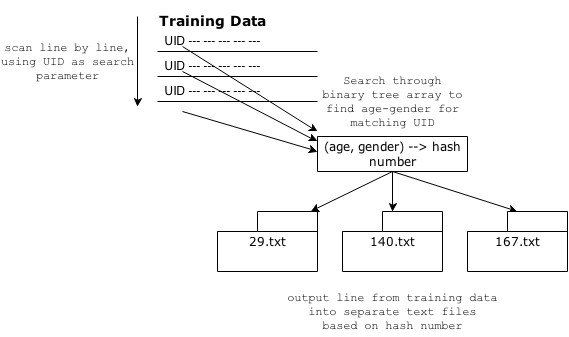
\includegraphics[scale=0.65]{TrainingData.png}

\subsection{Calculate the CTR}
Once the training data splitting is complete, we will go through each file and merge the results by AdID. We will add up all the impressions and clicks of matching AdID and sum them up. Then CTR can be calculated by dividing number of total clicks into total number of impressions. 

(This step is still on-going.)

\section{Build the Model and Make Prediction}
\subsection{Build the Model}
We will organize each hash group by title category, then we will use a logistic regression model to simulate pCTR using calculated CTR of each image as the y variable and the image features as the x variables. After logistic regression there should be a weight attached to each variable, and they will be used to calculcate pCTR of the testing data. 
\begin{center}
\begin{equation}
\begin{split}Logistic\,Model (Hash \,\#, \,Ad Cateogry)& = Image \,Features(f_1, f_2, f_3, ..., f_7) \backsim CTR_{calculated} \\&  \Rightarrow (w_1, w_2, ...,w_7)_{Hash \,\#}, _{Ad \,Category}
\end{split}
\end{equation}
\end{center}

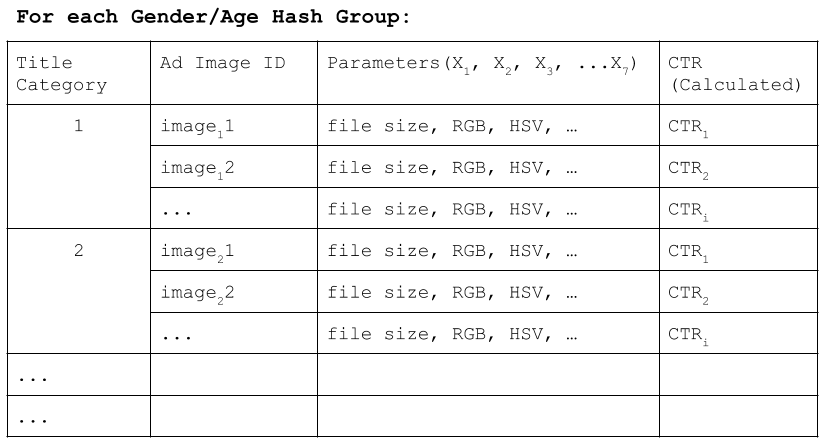
\includegraphics[scale=0.66]{Hash_Group_Model.png}

\subsection{Validate Model and Make Prediction}
To validate the model and make predictions, we plan to apply the Model we made to the splited evaluation dataset and validation dataset, and worked out the pCTR for different advertisements (based on title category and image features) and users from different gender and age groups, and then make a summary to test whether the pCTR is accurate.

(This step is still on-going.)

\section{Software Used}
The project will use, primarily, Java, Microsoft Excel, MySQL, and MatLab. Depending on future considerations for calculation efficiency and convenience, software capable of heavy mathematical modeling and computation will be required. Java will be used mainly for application-side utilities.

\section{References}
Bayesian Statistics
 
\url{http://www.maths.nott.ac.uk/personal/tk/files/talks/nott_radiology_01_11.pdf}

Gaussian Process

\url{http://citeseerx.ist.psu.edu/viewdoc/download?doi=10.1.1.84.1226&rep=rep1&type=pdf}

Nearest Neighbor Algorithm

 \url{http://citeseerx.ist.psu.edu/viewdoc/summary?doi=10.1.1.31.1422}

Machine Learning

\url{http://www.cs.nyu.edu/~mohri/mlbook/}



\end{document}
